\section{Background} \label{sec:Background}

\subsection{Game Software Engineering}
Video games present characteristics that differentiate their development
and maintenance from the development and maintenance
of classic software; for example, how developers contribute to video
games vs. non-games by working on different kinds of artifacts (e.g.,
shaders, meshes, or prefabs). In addition, game developers perceive
more difficulties than other non-game developers when locating
bugs as well as reusing code~\cite{pascarella2018video}.

Nowadays, most video games are developed by means of so called game engines. A game engine refers to a development environment that integrates a graphics engine and a physics engine as well as a set of tools that wraps around them in order to accelerate development. The most popular ones are Unity~\footnote{\url{https://unity.com/}} and Unreal Engine~\footnote{\url{https://www.unrealengine.com/}}, but it is also possible for a studio to make its own specific engine (e.g., CryEngine~\footnote{\url{https://www.cryengine.com}}).

A key artifact of game engines are software models. Developers can create video game content directly using code (e.g., C++) or the software models of the engines. On the one hand, the code allows developers to have more control over the content. On the other hand, software models are much less bound to the underlying implementation and technology and raise the abstraction level using terms that are much closer to the problem domain. This means that developers are liberated from a significant part of the implementation details of physics and graphics and can focus on the content of the game itself (see Figure~\ref{fig:architecture}). Unity and Unreal propose their own modeling language, and a recent survey in Model-Driven Game Development~\cite{zhu2019model} reveals that UML and Domain Specific Language (DSL) models are also adopted by development teams.

\begin{figure}[h]
    \centering
    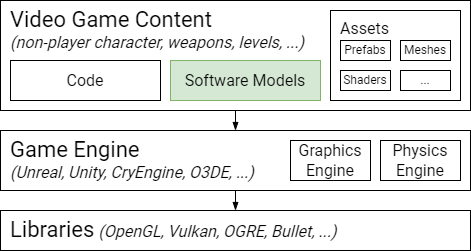
\includegraphics[width=0.45\textwidth]{Figures/ArchitectureLayers.drawio.png}
    \caption{Overview of video game artifacts. Highlighted in green Software Models, where this work focus.}
    \label{fig:architecture}
\end{figure}

\subsection{Case Study: \CaseStudy{}}
\label{subsec:case_study}

The case study that we use to evaluate the work presented here is
performed using the bosses of the video game Kromaia. The game
in Kromaia takes place in a three-dimensional space. Each of the
levels involves a player’s spaceship flying from a starting point to
a target destination reaching the goal before being destroyed. The
level involves exploring floating structures, avoiding asteroids, and
finding items along the route, while protected by basic enemies
that try to damage the player’s spaceship by firing projectiles. If
the player manages to reach the destination, the final boss corresponding
to that level appears and must be defeated in order to
complete the level.

The bosses are specified with the Shooter Definition Model Language
(SDML). SDML is a DSL model for the video game domain.
This DSL follows the main ideas of MDE using models for Software
Engineering. The models are created using SDML and interpreted
at runtime. Specifically, SDML defines aspects that are included
in video game entities: the anatomical structure (including which
parts are used in it, their physical properties, and how they are
connected to each other); the amount and distribution of vulnerable
parts, weapons, and defenses in the structure/body of the character;
and the movement behaviours associated to the whole body or its
parts. This modeling language has concepts such as hulls, links,
weak points, weapons, and AI components. Examples of the models,
the metamodel, and an online visualizer to show the models as
they would be seen in the Kromaia video game can be found at the
following URL: https://svit.usj.es/models22/bl-in-mgse. \todo{Modify link}

The simulations used in this work simulate a duel between a boss and a human player. The simulated player is an algorithm that is able
to act like a human player. It was created by the developers of the
Kromaia video game. We used their algorithm for our approach.
During the simulation, the simulated player faces the boss in order
to destroy the weak points that are available at that moment,
whereas the boss acts according to the anatomy, behaviour, and
attack/defense balance that is included in its model, trying to defeat
the simulated player. In the simulation, both the boss and the
simulated player try to win the match and do not avoid confrontation,
try to prevent draw/tie games, and try to ensure that there
is a winner. The algorithm can fight a boss by applying different
strategies. Hence, the algorithm can be parametrized to define the
fighting strategy. The simulation parameters were provided by the
developers based on the analysis of battles between human players
and bosses.

It is important to clarify that bosses can be built either using
SDML software models or directly with C++. The intuition of the
developers is that they make fewer mistakes and are more efficient
working with the models than with the code, and an experiment
confirmed this [15]. \mar{check if the clarification of models and code is in other part, if not adapt it. The part of the mistakes should not be relevant to our work.}